% Options for packages loaded elsewhere
% Options for packages loaded elsewhere
\PassOptionsToPackage{unicode}{hyperref}
\PassOptionsToPackage{hyphens}{url}
\PassOptionsToPackage{dvipsnames,svgnames,x11names}{xcolor}
%
\documentclass[
  letterpaper,
  DIV=11,
  numbers=noendperiod]{scrartcl}
\usepackage{xcolor}
\usepackage{amsmath,amssymb}
\setcounter{secnumdepth}{-\maxdimen} % remove section numbering
\usepackage{iftex}
\ifPDFTeX
  \usepackage[T1]{fontenc}
  \usepackage[utf8]{inputenc}
  \usepackage{textcomp} % provide euro and other symbols
\else % if luatex or xetex
  \usepackage{unicode-math} % this also loads fontspec
  \defaultfontfeatures{Scale=MatchLowercase}
  \defaultfontfeatures[\rmfamily]{Ligatures=TeX,Scale=1}
\fi
\usepackage{lmodern}
\ifPDFTeX\else
  % xetex/luatex font selection
  \setmainfont[Path=C:/Windows/Fonts/,Extension=.ttf,UprightFont=KoPubWorld
Dotum Medium,BoldFont=KoPubWorld Dotum Bold]{KoPubWorldDotum}
\fi
% Use upquote if available, for straight quotes in verbatim environments
\IfFileExists{upquote.sty}{\usepackage{upquote}}{}
\IfFileExists{microtype.sty}{% use microtype if available
  \usepackage[]{microtype}
  \UseMicrotypeSet[protrusion]{basicmath} % disable protrusion for tt fonts
}{}
\makeatletter
\@ifundefined{KOMAClassName}{% if non-KOMA class
  \IfFileExists{parskip.sty}{%
    \usepackage{parskip}
  }{% else
    \setlength{\parindent}{0pt}
    \setlength{\parskip}{6pt plus 2pt minus 1pt}}
}{% if KOMA class
  \KOMAoptions{parskip=half}}
\makeatother
% Make \paragraph and \subparagraph free-standing
\makeatletter
\ifx\paragraph\undefined\else
  \let\oldparagraph\paragraph
  \renewcommand{\paragraph}{
    \@ifstar
      \xxxParagraphStar
      \xxxParagraphNoStar
  }
  \newcommand{\xxxParagraphStar}[1]{\oldparagraph*{#1}\mbox{}}
  \newcommand{\xxxParagraphNoStar}[1]{\oldparagraph{#1}\mbox{}}
\fi
\ifx\subparagraph\undefined\else
  \let\oldsubparagraph\subparagraph
  \renewcommand{\subparagraph}{
    \@ifstar
      \xxxSubParagraphStar
      \xxxSubParagraphNoStar
  }
  \newcommand{\xxxSubParagraphStar}[1]{\oldsubparagraph*{#1}\mbox{}}
  \newcommand{\xxxSubParagraphNoStar}[1]{\oldsubparagraph{#1}\mbox{}}
\fi
\makeatother


\usepackage{longtable,booktabs,array}
\newcounter{none} % for unnumbered tables
\usepackage{calc} % for calculating minipage widths
% Correct order of tables after \paragraph or \subparagraph
\usepackage{etoolbox}
\makeatletter
\patchcmd\longtable{\par}{\if@noskipsec\mbox{}\fi\par}{}{}
\makeatother
% Allow footnotes in longtable head/foot
\IfFileExists{footnotehyper.sty}{\usepackage{footnotehyper}}{\usepackage{footnote}}
\makesavenoteenv{longtable}
\usepackage{graphicx}
\makeatletter
\newsavebox\pandoc@box
\newcommand*\pandocbounded[1]{% scales image to fit in text height/width
  \sbox\pandoc@box{#1}%
  \Gscale@div\@tempa{\textheight}{\dimexpr\ht\pandoc@box+\dp\pandoc@box\relax}%
  \Gscale@div\@tempb{\linewidth}{\wd\pandoc@box}%
  \ifdim\@tempb\p@<\@tempa\p@\let\@tempa\@tempb\fi% select the smaller of both
  \ifdim\@tempa\p@<\p@\scalebox{\@tempa}{\usebox\pandoc@box}%
  \else\usebox{\pandoc@box}%
  \fi%
}
% Set default figure placement to htbp
\def\fps@figure{htbp}
\makeatother





\setlength{\emergencystretch}{3em} % prevent overfull lines

\providecommand{\tightlist}{%
  \setlength{\itemsep}{0pt}\setlength{\parskip}{0pt}}



 


\usepackage{emoji}
\setemojifont{Segoe UI Emoji}
\KOMAoption{captions}{tableheading}
\makeatletter
\@ifpackageloaded{caption}{}{\usepackage{caption}}
\AtBeginDocument{%
\ifdefined\contentsname
  \renewcommand*\contentsname{Table of contents}
\else
  \newcommand\contentsname{Table of contents}
\fi
\ifdefined\listfigurename
  \renewcommand*\listfigurename{List of Figures}
\else
  \newcommand\listfigurename{List of Figures}
\fi
\ifdefined\listtablename
  \renewcommand*\listtablename{List of Tables}
\else
  \newcommand\listtablename{List of Tables}
\fi
\ifdefined\figurename
  \renewcommand*\figurename{Figure}
\else
  \newcommand\figurename{Figure}
\fi
\ifdefined\tablename
  \renewcommand*\tablename{Table}
\else
  \newcommand\tablename{Table}
\fi
}
\@ifpackageloaded{float}{}{\usepackage{float}}
\floatstyle{ruled}
\@ifundefined{c@chapter}{\newfloat{codelisting}{h}{lop}}{\newfloat{codelisting}{h}{lop}[chapter]}
\floatname{codelisting}{Listing}
\newcommand*\listoflistings{\listof{codelisting}{List of Listings}}
\makeatother
\makeatletter
\makeatother
\makeatletter
\@ifpackageloaded{caption}{}{\usepackage{caption}}
\@ifpackageloaded{subcaption}{}{\usepackage{subcaption}}
\makeatother
\usepackage{bookmark}
\IfFileExists{xurl.sty}{\usepackage{xurl}}{} % add URL line breaks if available
\urlstyle{same}
\hypersetup{
  pdftitle={Rscript 활용하기},
  pdfauthor={Eunji Ha},
  colorlinks=true,
  linkcolor={blue},
  filecolor={Maroon},
  citecolor={Blue},
  urlcolor={Blue},
  pdfcreator={LaTeX via pandoc}}


\title{Rscript 활용하기}
\usepackage{etoolbox}
\makeatletter
\providecommand{\subtitle}[1]{% add subtitle to \maketitle
  \apptocmd{\@title}{\par {\large #1 \par}}{}{}
}
\makeatother
\subtitle{효율적인 연구를 위한}
\author{Eunji Ha}
\date{}
\begin{document}
\maketitle


본 강의에서는 ``배운 R 기초를 어떻게 실제 논문 작성에 써먹는가''에
집중하고자 합니다.

단순히 코드를 입력하는 수준을 넘어, 데이터 입력(Input) 시 논문용 표와
그래프(Output)가 자동으로 생성되는 실무 파이프라인 구축을 목표로 합니다.

\subsection{Part1. 연구 효율을 높이는 R script 환경
구축}\label{part1.-uxc5f0uxad6c-uxd6a8uxc728uxc744-uxb192uxc774uxb294-r-script-uxd658uxacbd-uxad6cuxcd95}

기초를 배운 직후이므로, R을 실제 연구 도구로 세팅하는 법부터 시작합니다.

\begin{itemize}
\item
  \textbf{R script 활용 파이프라인 구축?}

  input: 연구 데이터 ➡️ \textbf{R script} ➡️ output: 논문용 표 \&
  그래프📊📈

  ✅ 휴먼 에러 최소화

  ✅ 연구 효율성

  ✅ Reproducibility
\item
  \textbf{R 프로젝트 파일 관리}: 폴더 구조 체계화

  \begin{itemize}
  \item
    \texttt{scripts/}: 전처리 및 분석용 스크립트 관리
  \item
    \texttt{rawdata/}: 원본 데이터 (+다른 곳에 백업)
  \item
    \texttt{analysis/}: 단계별 분석 결과 저장
  \item
    \texttt{results/}: 최종 Table 및 고해상도 Figure 정리

    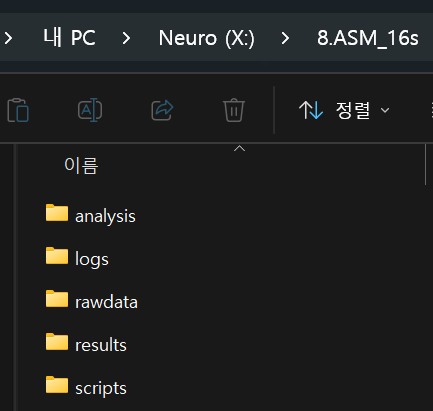
\includegraphics[width=3.51042in,height=\textheight,keepaspectratio]{images/clipboard-3256079201.png}
  \end{itemize}
\end{itemize}

\subsection{Part2. R script 활용 분석 파이프라인
이해}\label{part2.-r-script-uxd65cuxc6a9-uxbd84uxc11d-uxd30cuxc774uxd504uxb77cuxc778-uxc774uxd574}

\begin{itemize}
\tightlist
\item
  CSV/xlsx 읽기 → 전처리 → Table 1 (gtsummary) → KM → Cox → forest plot
\item
  \textbf{데이터 전처리 (The Tidy Way)}: 엑셀에서 하던 필터링과 정렬을
  \texttt{dplyr} 패키지로 자동화하며, 이 과정이 전체의 70\%임을
  공유합니다.
\item
  \textbf{Table 1 자동 생성 (\texttt{tableone}, \texttt{gtsummary})}:

  \begin{itemize}
  \tightlist
  \item
    연속형/범주형 변수를 자동 판별하고 p-value를 한 번에 계산하는 실습을
    진행합니다.
  \item
    \textbf{Labeling 기법}: 변수명(\texttt{sbp\_v1})을 출력용
    이름(\texttt{Systolic\ BP})으로 자동 변환하여 `복사-붙여넣기'
    수작업을 생략합니다.
  \end{itemize}
\item
  \textbf{바이브코딩으로 R 스크립트 만들기} - AI에게 프롬프트 → 코드
  생성 → 실행 → 수정 사이클 - 좋은 프롬프트 작성법, AI가 틀리기 쉬운
  통계적 함정
\end{itemize}

\subsection{Part3. 결과 시각화 및 전문 리포팅 / 참가자 실습 +
마무리}\label{part3.-uxacb0uxacfc-uxc2dcuxac01uxd654-uxbc0f-uxc804uxbb38-uxb9acuxd3ecuxd305-uxcc38uxac00uxc790-uxc2e4uxc2b5-uxb9c8uxbb34uxb9ac}

\begin{itemize}
\tightlist
\item
  \textbf{핵심 Figure 그리기}: 논문의 퀄리티를 결정짓는
  \textbf{Kaplan-Meier Curve}나 \textbf{Forest Plot}을 생성
\item
  \textbf{통계 수치 자동 추출}: p-value, HR, CI 등을 직접 타이핑하지
  않고 \texttt{broom} 패키지를 통해 오타 없이 데이터프레임으로 추출
\item
  \textbf{Quarto를 활용한 `원클릭 보고서'}: 분석 코드와 해석이 포함된
  문서를 PDF/Word/HTML로 즉시 출력하여 PI 보고용 자료를 완성
\item
  R Markdown으로 재현 가능한 리포트
\item
  \textbf{맞춤형 템플릿 제공}: 생존분석(Survival Analysis)이나 성향점수
  매칭(PSM) 등 실제 연구 주제에 맞춘 \textbf{``Ready-to-use''}
  스크립트를 배포하여 즉시 활용 가능하게 합니다.
\item
  \textbf{성공 경험 중심}: 이론 설명은 10\% 이내로 줄이고,
  \textbf{``데이터 넣기 → 코드 실행 → 결과 확인''} 과정을 반복하여
  효용을 직접 느끼게 하는 것이 중요합니다.
\end{itemize}

\begin{quote}
\textbf{AI 활용 가이드 (Magic Prompt)}: ``나는 간암 환자 200명의 생존
분석을 하고 있어. 데이터프레임 \texttt{df}를 사용해서 Kaplan-Meier
곡선을 그려주고, Risk Table과 Log-rank test p-value를 포함해줘
\end{quote}




\end{document}
